% style.tex -- shared preamble for the standalone test reports.
%
% Each report is an independent document: build it with
%   latexmk -xelatex -interaction=nonstopmode -halt-on-error -outdir=build <file>.tex
% from the reports/ directory. The main project report is intentionally not
% part of this directory; these reports document the test evidence on its own.

\documentclass[UTF8,a4paper,11pt]{ctexart}

\usepackage{geometry}
\geometry{top=2.3cm,bottom=2.3cm,left=2.5cm,right=2.5cm,headheight=14pt}

\usepackage{fontspec}
\setmainfont{DejaVu Serif}[AutoFakeSlant=0.2]
\setsansfont{DejaVu Sans}[AutoFakeSlant=0.2]
\setmonofont{DejaVu Sans Mono}[Scale=0.88]

\usepackage{amsmath,amssymb}
\usepackage{graphicx}
\graphicspath{{figures/}}
\usepackage{booktabs}
\usepackage{tabularx}
\usepackage{longtable}
\usepackage{array}
\usepackage{enumitem}
\usepackage{caption}
\usepackage{float}
\usepackage{xcolor}
\usepackage{listings}
\usepackage{fancyhdr}
\usepackage{hyperref}

\definecolor{codebg}{gray}{0.96}
\definecolor{codeframe}{gray}{0.45}
\lstset{
  basicstyle=\ttfamily\small,
  breaklines=true,
  breakatwhitespace=true,
  columns=fullflexible,
  keepspaces=true,
  frame=single,
  framerule=0.3pt,
  rulecolor=\color{codeframe},
  backgroundcolor=\color{codebg},
  showstringspaces=false,
  tabsize=2,
  aboveskip=0.7em,
  belowskip=0.7em,
}

% Inline code. detokenize preserves spaces and special characters; a plain
% lstinline argument loses spaces under ctex (xeCJK-listings turns them into
% CJK glue). Avoid a literal percent sign in the argument.
\newcommand{\code}[1]{\texttt{\detokenize{#1}}}

\pagestyle{fancy}
\fancyhf{}
\fancyhead[L]{\small 迷你搜索引擎项目}
\fancyhead[R]{\small 测试报告}
\fancyfoot[C]{\thepage}
\renewcommand{\headrulewidth}{0.4pt}
\fancypagestyle{plain}{%
  \fancyhf{}%
  \fancyfoot[C]{\thepage}%
  \renewcommand{\headrulewidth}{0pt}%
}

\captionsetup{font=small,labelfont=bf,skip=5pt}
\setlength{\parskip}{0.35em}
\setlength{\parindent}{2em}
\setlength{\emergencystretch}{3em}
\renewcommand{\arraystretch}{1.15}
\setlist{itemsep=0.2em,topsep=0.3em}

\hypersetup{
  colorlinks=true,
  linkcolor=blue!55!black,
  urlcolor=blue!55!black,
  bookmarksnumbered=true,
}

% Report title block: number/title, subtitle, version.
\newcommand{\reportheader}[3]{%
  \begin{center}
    {\large 迷你搜索引擎项目}\\[0.35em]
    {\LARGE\bfseries #1}\\[0.45em]
    {\large #2}\\[0.6em]
    {\small 版本 #3 \quad 测试日期 2026-10-19}
  \end{center}
  \vspace{0.3em}
  \noindent\rule{\linewidth}{0.6pt}
  \vspace{0.8em}
}

% A highlighted conclusion.
\newcommand{\finding}[1]{%
  \begin{quote}
    \noindent\textbf{结论：}#1
  \end{quote}
}


\begin{document}

\reportheader{测试报告 03：查询阈值实验}{四个阈值对结果集的影响（201 条测量）}{1.0}
\hypersetup{pdftitle={测试报告 03：查询阈值实验}}

\begin{center}\small
\begin{tabularx}{0.92\linewidth}{@{}l X@{}}
  报告编号 & TR-03 \\
  被测对象 & \code{mse query} 的四个阈值 \\
  被测版本 & 分支 \code{test/reports}，基于 \code{origin/main} 加注释与测试改动 \\
  测试环境 & WSL2（Linux 6.18），g++ 15.2，Python 3；正式索引（stopwords + stem） \\
  测试日期 & 2026-10-19 \\
  总体结论 & 201 条测量全部完成；四类阈值的作用位置与副作用已量化 \\
\end{tabularx}
\end{center}

\section{目标与范围}

本报告量化 \code{mse query} 的四个阈值：

\begin{itemize}
  \item \code{--max-df}：丢弃“太大众”的查询词；
  \item \code{--min-df}：丢弃太罕见的查询词；
  \item \code{--min-match}：布尔查询至少命中几个词；
  \item \code{--top-x}：只保留得分最高的前 $x$ 篇文档。
\end{itemize}

实验回答三个问题：阈值把结果集改变了多少、改变发生在“词侧”还是“结果侧”、不同查询类型对阈值的敏感度是否相同。

\section{方法}

\subsection{查询集}

固定 15 条查询，覆盖 8 类查询意图（表~\ref{tab:queries}）。查询集不随机生成：它覆盖高频词、中频词、低频词、专名、短语、含停用词的短语、布尔组合与停用词，保证每个阈值都有可观察的边界。

\begin{table}[H]
  \centering
  \caption{阈值实验的查询集}
  \label{tab:queries}
  \small
  \begin{tabularx}{\linewidth}{@{}l l X@{}}
    \toprule
    查询 & 类别 & 选择理由 \\
    \midrule
    \code{love} & high & $df\_ratio$ 0.71，高频内容词 \\
    \code{sweet} & high & $df\_ratio$ 0.46 \\
    \code{good} & mid & $df\_ratio$ 0.29 \\
    \code{night} & mid & $df\_ratio$ 0.29 \\
    \code{sword} & low & $df=37$ \\
    \code{moon} & low & $df=35$ \\
    \code{banquo} & name & $df=1$，专名 \\
    \code{osric} & name & $df=1$，专名 \\
    \code{king queen} & bool & 两个中频词，AND 基线 \\
    \code{sweet sword moon} & bool & 三个词，观察丢词后的“放宽” \\
    \code{good night} & phrase & 普通短语 \\
    \code{king richard} & phrase & 结果较少的短语（7 篇） \\
    \code{my lord} & phrase-stop & \code{my} 是停用词，短语退化 \\
    \code{the} & stopword & 过滤索引中不可检索 \\
    \code{of} & stopword & 过滤索引中不可检索 \\
    \bottomrule
  \end{tabularx}
\end{table}

\subsection{测量协议}

每次只改变一个参数，其余阈值保持关闭（基线）。每条测量记录：

\begin{itemize}
  \item 返回文档数；
  \item 与基线的 Jaccard 相似度 $J=|A\cap B|/|A\cup B|$；
  \item note 数（解释被丢弃的词、停用词等）；
  \item 查询耗时（毫秒）。
\end{itemize}

共 $15$ 条基线 $+75$ 条 \code{--max-df} $+60$ 条 \code{--min-df} $+6$ 条 \code{--min-match} $+45$ 条 \code{--top-x} $=\mathbf{201}$ 条测量。原始数据保存在 \code{data/threshold_matrix.csv}，生成脚本为 \code{tools/threshold_matrix.py}。

\section{结果}

\subsection{\texttt{--max-df}：丢弃“太大众”的词}

\begin{table}[H]
  \centering
  \caption{\texttt{--max-df} 扫描（单元格为返回文档数）}
  \label{tab:max-df}
  \small
  \begin{tabularx}{\linewidth}{@{}X r r r r r r@{}}
    \toprule
    查询 & 基线 & 0.9 & 0.7 & 0.5 & 0.3 & 0.1 \\
    \midrule
    love（0.71） & 138 & 138 & 0 & 0 & 0 & 0 \\
    sweet（0.46） & 90 & 90 & 90 & 90 & 0 & 0 \\
    good（0.29） & 57 & 57 & 57 & 57 & 57 & 0 \\
    night（0.29） & 56 & 56 & 56 & 56 & 56 & 0 \\
    sword（0.19） & 37 & 37 & 37 & 37 & 37 & 0 \\
    moon（0.18） & 35 & 35 & 35 & 35 & 35 & 0 \\
    banquo / osric（$df=1$） & 1 & 1 & 1 & 1 & 1 & 1 \\
    king queen & 33 & 33 & 33 & 33 & 33 & 0 \\
    sweet sword moon & 30 & 30 & 30 & 30 & 30 & 0 \\
    短语查询 & 7/23/42 & 7/23/42 & 7/23/42 & 7/23/42 & 7/23/42 & 7/23/42 \\
    the / of & 0 & 0 & 0 & 0 & 0 & 0 \\
    \bottomrule
  \end{tabularx}
\end{table}

\subsection{\texttt{--min-df}：丢弃太罕见的词}

\begin{table}[H]
  \centering
  \caption{\texttt{--min-df} 扫描}
  \label{tab:min-df}
  \small
  \begin{tabularx}{\linewidth}{@{}X r r r r r@{}}
    \toprule
    查询 & 基线 & 2 & 5 & 20 & 50 \\
    \midrule
    banquo / osric（$df=1$） & 1 & 0 & 0 & 0 & 0 \\
    sword（$df=37$） & 37 & 37 & 37 & 37 & 0 \\
    moon（$df=35$） & 35 & 35 & 35 & 35 & 0 \\
    king queen & 33 & 33 & 33 & 33 & 0 \\
    sweet sword moon & 30 & 30 & 30 & 30 & 90 \\
    \bottomrule
  \end{tabularx}
  \par\smallskip
  \footnotesize 注：最后一行在 \code{--min-df 50} 时丢弃了 \code{sword} 与 \code{moon}，只剩 \code{sweet}，结果从 30 篇增加到 90 篇；与基线的 Jaccard 为 0.33。
\end{table}

\subsection{\texttt{--min-match}：布尔语义的松紧}

\begin{table}[H]
  \centering
  \caption{\texttt{--min-match} 扫描（括号内为 Jaccard）}
  \label{tab:min-match}
  \small
  \begin{tabularx}{\linewidth}{@{}X r r r r@{}}
    \toprule
    查询 & 基线（AND） & $k=1$ & $k=2$ & $k=3$ \\
    \midrule
    king queen & 33 & 43（0.77） & 33 & 33 \\
    sweet sword moon & 30 & 93（0.32） & 39（0.77） & 30 \\
    \bottomrule
  \end{tabularx}
\end{table}

$k$ 超过可检索词数时会被钳制为词数，不会返回空集。表中 $k=3$ 对 \code{king queen}（两个词）等价于 AND。

\subsection{\texttt{--top-x}：结果截断}

\begin{table}[H]
  \centering
  \caption{\texttt{--top-x} 扫描（括号内为 Jaccard）}
  \label{tab:top-x}
  \small
  \begin{tabularx}{\linewidth}{@{}X r r r r@{}}
    \toprule
    查询 & 基线 & 5 & 10 & 20 \\
    \midrule
    love & 138 & 5（0.04） & 10（0.07） & 20（0.14） \\
    good night & 23 & 5（0.22） & 10（0.43） & 20（0.87） \\
    king richard & 7 & 5（0.71） & 7（1.00） & 7（1.00） \\
    banquo / osric & 1 & 1（1.00） & 1（1.00） & 1（1.00） \\
    \bottomrule
  \end{tabularx}
\end{table}

\begin{figure}[H]
  \centering
  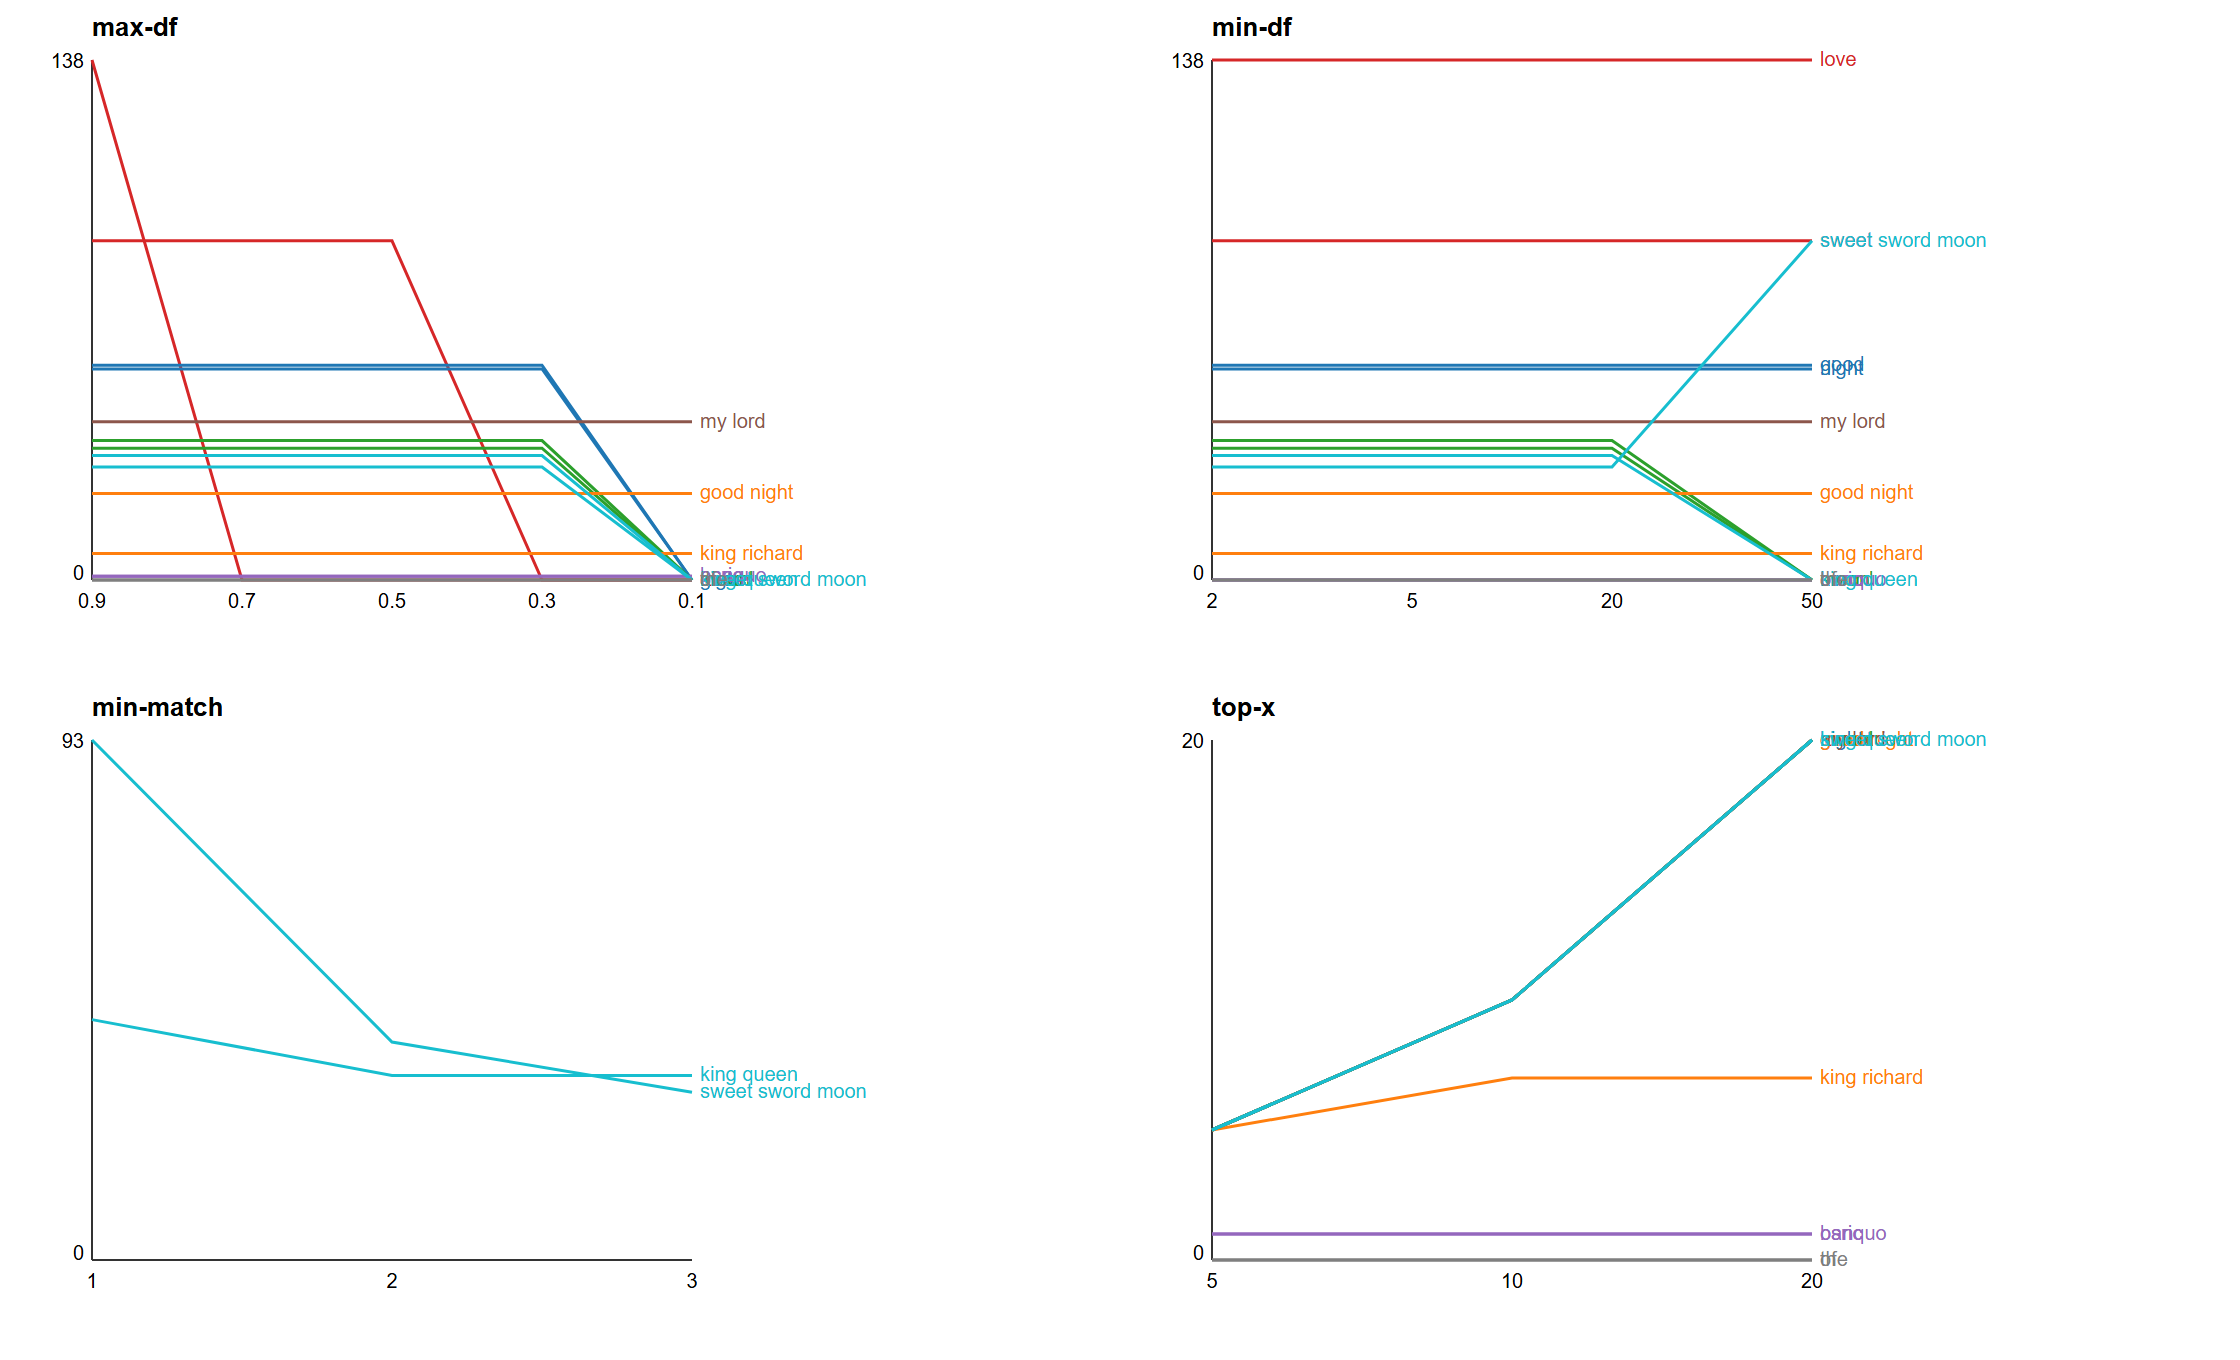
\includegraphics[width=\linewidth]{figures/threshold_matrix.png}
  \caption{阈值矩阵：每个面板一个参数，横轴为参数值，纵轴为返回文档数。}
  \label{fig:matrix}
\end{figure}

\section{分析}

\begin{enumerate}
  \item \textbf{\texttt{--max-df} 直接消除高频词的结果。} 单词查询一旦词被丢弃，结果从上百篇直接归零。\code{love} 在 0.7 档（$df\_ratio$ 0.71）被丢弃，\code{sweet} 在 0.3 档被丢弃。阈值必须按查询意图设定，不能一律取小。
  \item \textbf{\texttt{--min-df} 与多词 AND 组合会产生“丢词即放宽”。} \code{sweet sword moon} 在 \code{--min-df 50} 下丢弃 \code{sword} 与 \code{moon}，只剩 \code{sweet}，结果从 30 篇增加到 90 篇，Jaccard 仅 0.33。原因是阈值作用于查询词，而不是直接作用于结果文档。
  \item \textbf{\texttt{--min-match} 是布尔语义的旋钮。} $k=1$ 即 OR，结果集显著扩大；$k=\text{词数}$ 即 AND；超过词数时钳制，不会返回空集。
  \item \textbf{\texttt{--top-x} 是纯结果侧截断。} 它不改变匹配语义，Jaccard 随 $x$ 单调回升；对结果数不超过 $x$ 的查询没有影响。
  \item \textbf{短语查询不受词侧阈值影响。} 7/23/42 三组短语结果在所有 \code{--max-df} 档位保持不变（Jaccard 恒 1.00）。这是设计行为：短语是整体，丢掉任何一个词都不再是原短语。
  \item \textbf{停用词查询恒为空。} 过滤索引中 \code{the}/\code{of} 没有 posting，与阈值无关；系统输出 note 解释原因。
\end{enumerate}

\section{复现方式}

\begin{lstlisting}[language=bash]
# 重新生成 201 条测量与图
python3 tools/threshold_matrix.py

# 产物
#   build/threshold_matrix.csv   原始测量
#   build/threshold_matrix.svg   图
\end{lstlisting}

CSV 列为 \code{query, category, mode, param, value, results, jaccard, notes, ms}。本报告使用的 CSV 副本在 \code{reports/data/threshold_matrix.csv}，可以直接用任意表格工具复查表~\ref{tab:max-df}–\ref{tab:top-x}。

\section{结论与建议}

\begin{itemize}
  \item 四个阈值分别作用于“词侧”（\code{--max-df}、\code{--min-df}）、“匹配语义”（\code{--min-match}）和“结果侧”（\code{--top-x}），不能用同一个“召回率”口径解释；
  \item 默认配置应保持所有阈值关闭，让查询语义可预测；需要降噪时优先用 \code{--max-df}，但必须接受高频词查询归零；
  \item \code{--min-df} 与多词 AND 组合存在反直觉的“结果变多”现象，交互式系统应提示被丢弃的词；
  \item \code{--top-x} 适合展示层截断，不适合作为召回率优化手段；
  \item 短语查询应保持“整段匹配”，不要对短语应用词侧阈值。
\end{itemize}

\finding{阈值不是“越小越好”的过滤器，而是改变查询语义的四个旋钮；本实验用 201 条测量给出了每个旋钮的作用位置和副作用。}

\end{document}
